\documentclass[10pt,a4paper]{article}
%\usepackage[latin1]{inputenc}
\usepackage{amsmath}
\usepackage{amsfonts}
\usepackage{amssymb}
\usepackage{graphicx}
\usepackage[left=0.50cm, right=0.50cm, top=0.50cm, bottom=0.50cm]{geometry}
\begin{document}
	\textbf{Given}: $$A \sim N(\mu_A, \sigma_A), B \sim N(\mu_B, \sigma_B), 0 < \mu_A < \mu_B, 0 < \alpha < 1$$
	
	\textbf{Evaluate}: $$\mathop{\arg\min}_{\mu_A < T < \mu_B}\ \alpha \cdot \int_{-\infty}^{T}P_B(x)dx + (1 - \alpha) \cdot \int_{T}^{+\infty}P_A(x)dx$$
	
	\begin{figure}[!ht]
		\centering
		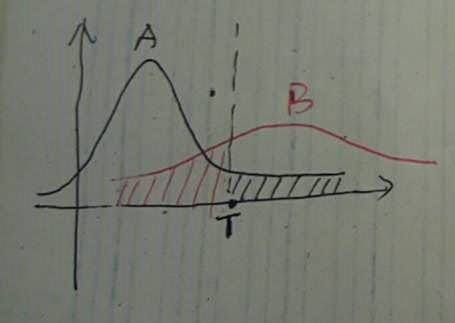
\includegraphics[width=0.5\linewidth]{SamplePic.jpg}
	\end{figure}
	
	Let:
	\begin{equation}
		\begin{split}
		g(T) & = \alpha \cdot \int_{-\infty}^{T}P_B(x)dx + (1 - \alpha) \cdot \int_{T}^{+\infty}P_A(x)dx \ ,\ \mu_A < T < \mu_B\\
		& = \alpha \cdot \int_{-\infty}^{T}P_B(x)dx + (1 - \alpha) \cdot \Big(1 - \int_{-\infty}^{T}P_A(x)dx\Big) \ ,\ \mu_A < T < \mu_B
		\end{split}
	\end{equation}
	
	%According to cumulative function of normal distribution:
	%$$F(x) = \frac{1}{2}\Big[1 + erf\big(\frac{x - \mu}{\sigma\sqrt{2}}\big)\Big]$$
	%
	%where $erf(x)$ is the error function:
	%
	%$$erf(x) = \frac{2}{\sqrt{\pi}}\int_{0}^{x}e^{-t^2}dt$$
	%
	%$$erf'(x) = \frac{2}{\sqrt{\pi}}e^{-x^2}$$
	
	Then:
	
	%\begin{equation}
	%\begin{split}
	%	g(T) & = \alpha F_B(T) + (1 - \alpha) F_A(2\mu_A - T)\\
	%	& = \frac{\alpha}{2}\Big[1 + erf\big(\frac{T - \mu_B}{\sigma_B\sqrt{2}}\big)\Big] + \frac{1 - \alpha}{2}\Big[1 + erf\big(\frac{\mu_A - T}{\sigma_A\sqrt{2}}\big)\Big]
	%\end{split}
	%\end{equation}
	
	\begin{equation}\label{equ:1st-drv}
		\begin{split}
		g'(T) & = \alpha P_B(T) - (1 - \alpha) P_A(T)\\
		%g'(T) & = \frac{\alpha}{2}erf'\big(\frac{T - \mu_B}{\sigma_B\sqrt{2}}\big) + \frac{1 - \alpha}{2}erf'\big(\frac{\mu_A - T}{\sigma_A\sqrt{2}}\big)\\
		%& = \frac{\alpha}{\sqrt{\pi}}e^{-(\frac{T - \mu_B}{\sigma_B\sqrt{2}})^2}
		%\cdot \frac{1}{\sigma_B\sqrt{2}}
		%+ \frac{1 - \alpha}{\sqrt{\pi}}e^{-(\frac{\mu_A - T}{\sigma_A\sqrt{2}})^2}
		%\cdot \frac{-1}{\sigma_A\sqrt{2}}\\
		& = \frac{\alpha}{\sigma_B\sqrt{2\pi}}e^{-(\frac{T - \mu_B}{\sigma_B\sqrt{2}})^2}
		- \frac{1 - \alpha}{\sigma_A\sqrt{2\pi}}e^{-(\frac{\mu_A - T}{\sigma_A\sqrt{2}})^2}
		\end{split}
	\end{equation}
	
	\begin{equation}\label{equ:2nd-drv}
		\begin{split}
		g''(T) & = \frac{\alpha}{\sigma_B\sqrt{2\pi}}
		e^{-(\frac{T - \mu_B}{\sigma_B\sqrt{2}})^2} \cdot (-2) \cdot 
		\frac{T - \mu_B}{\sigma_B\sqrt{2}} \cdot \frac{1}{\sigma_B\sqrt{2}}
		- \frac{1 - \alpha}{\sigma_A\sqrt{2\pi}}
		e^{-(\frac{\mu_A - T}{\sigma_A\sqrt{2}})^2} \cdot (-2) \cdot 
		\frac{\mu_A - T}{\sigma_A\sqrt{2}} \cdot \frac{-1}{\sigma_A\sqrt{2}}\\
		& = \frac{\alpha(\mu_B - T)}{\sigma_B^3\sqrt{2\pi}}
		e^{-(\frac{T - \mu_B}{\sigma_B\sqrt{2}})^2}
		+ \frac{(1 - \alpha)(T - \mu_A)}{\sigma_A^3\sqrt{2\pi}}
		e^{-(\frac{\mu_A - T}{\sigma_A\sqrt{2}})^2}
		\end{split}
	\end{equation}
	
	According to (\ref{equ:2nd-drv}), $g''(T) > 0$ for $\forall T \in (\mu_A, \mu_B)$
	
	According to (\ref{equ:1st-drv}), 
	
	\begin{equation}
		\left.
		\begin{aligned}
		g'(\mu_A) < 0\\
		g'(\mu_B) > 0
		\end{aligned}
		\right\}
		\Rightarrow \frac{\sigma_B \cdot e^{-(\frac{\mu_A - \mu_B}{\sigma_A\sqrt{2}})^2}}{\sigma_A + \sigma_B \cdot 
		e^{-(\frac{\mu_A - \mu_B}{\sigma_A\sqrt{2}})^2}}
		< \alpha < \frac{\sigma_B}{\sigma_A \cdot 
		e^{-(\frac{\mu_A - \mu_B}{\sigma_B\sqrt{2}})^2} + \sigma_B}
	\end{equation}
	
	Let: $g'(T) = 0$
	
	Then:
	
	\begin{equation}
		\begin{split}
		\frac{\alpha}{\sigma_B\sqrt{2\pi}}e^{-(\frac{T - \mu_B}{\sigma_B\sqrt{2}})^2}
		& =  \frac{1 - \alpha}{\sigma_A\sqrt{2\pi}}e^{-(\frac{\mu_A - T}{\sigma_A\sqrt{2}})^2}\\
		ln\Big(\frac{\alpha}{\sigma_B}\Big) - \Big(\frac{T - \mu_B}{\sigma_B\sqrt{2}}\Big)^2
		& = ln\Big(\frac{1 - \alpha}{\sigma_A}\Big) - \Big(\frac{\mu_A - T}{\sigma_A\sqrt{2}}\Big)^2\\
		\end{split}
	\end{equation}
	
\end{document}








